% Shared preamble for the English summaries in this repository.
\documentclass[11pt,a4paper]{article}
\usepackage[margin=2.2cm]{geometry}
\usepackage[T1]{fontenc}
\usepackage[utf8]{inputenc}
\usepackage{lmodern}
\usepackage{amsmath,amssymb}
\usepackage{graphicx}
\usepackage{booktabs}
\usepackage{enumitem}
\usepackage[hidelinks]{hyperref}
\setlist{itemsep=2pt,topsep=4pt}
\setlength{\parindent}{0pt}
\setlength{\parskip}{5pt}
\graphicspath{{figures/}}
\newcommand{\summaryheader}[3]{%
  \begin{center}
    {\Large\bfseries #2}\\[3pt]
    {\large #1}\\[3pt]
    {\small Arshia Goshtasbi \textbullet{} MSc Electrical Engineering (Control), Iran University of Science and Technology \textbullet{} #3}
  \end{center}
  \vspace{2pt}\hrule\vspace{8pt}\par}

\begin{document}
\summaryheader{Machine Learning, Homework 7}{KNN and K-means from Scratch, and EM for a Coin Mixture}{Spring 1404 (2025)}

\textbf{Notebooks.}
\begin{itemize}
  \item \texttt{knn-from-scratch.ipynb}: the same employee-attrition data as HW3. I removed constant columns, one-hot encoded the categorical ones, made an 80/20 split and implemented KNN (Euclidean distance, majority vote) from scratch. With $K=5$ on unscaled features, my implementation and scikit-learn's \texttt{KNeighborsClassifier} give identical results: $0.821$ training and $0.762$ test accuracy.
  \item \texttt{kmeans-from-scratch.ipynb}: K-means from scratch on 4000 random rows of California Housing, compared with scikit-learn's \texttt{KMeans} using the elbow and silhouette methods (Figure~\ref{fig:km}). Both implementations give the same curves; the silhouette score is highest at $k=2$. I prefer the silhouette method because it gives a clear maximum, while the elbow is a judgement call.
\end{itemize}

\begin{figure}[h]\centering
  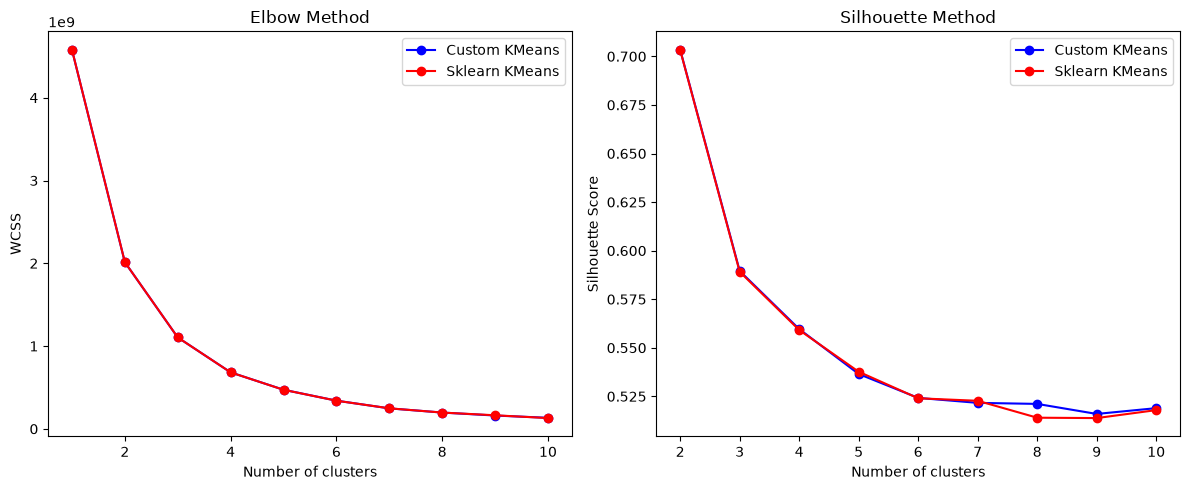
\includegraphics[width=.9\linewidth]{kmeans-from-scratch_cell14_1.png}
  \caption{Elbow (WCSS) and silhouette scores for my K-means and scikit-learn's.}\label{fig:km}
\end{figure}

\textbf{Written part.}
\begin{description}
  \item[KNN on a small 2D set.] I found the $K$ with the lowest training error and the lowest leave-one-out error, and drew the 1-NN decision boundary. A very small $K$ follows noise and outliers. A very large $K$ over-smooths and predicts the majority class everywhere.
  \item[K-means.] Each step does not increase $J$ and there are at most $k^n$ assignments $\gamma$, so the algorithm stops in finitely many steps. The total scatter splits as $T(X)=\sum_j\frac{n_j}{n}W_j(X)+B(X)$, so minimising the weighted within-cluster scatter is the same as maximising the between-cluster scatter $B$. The minimum of $J$ never increases with $k$ (it reaches $0$ at $k=n$), so $k$ cannot be chosen by minimising $J$.
  \item[EM for two biased coins.] With hidden coin choice $Z_i$ and $\theta=(\pi,p_r,p_b)$: $p(x,z;\theta)=\big[\pi p_r^x(1-p_r)^{1-x}\big]^z\big[(1-\pi)p_b^x(1-p_b)^{1-x}\big]^{1-z}$. If $z_i$ were known, the ML estimates are $\hat\pi=\frac1m\sum z_i$, $\hat p_r=\sum z_ix_i/\sum z_i$ and $\hat p_b=\sum(1-z_i)x_i/\sum(1-z_i)$. EM replaces $z_i$ by the posterior $\gamma_i=P(Z_i{=}1\mid x_i;\theta^\alpha)$ in the E-step and uses the same formulas with $\gamma_i$ in the M-step.
\end{description}
\end{document}
